\cleardoublepage
\newpage
\ThisULCornerWallPaper{1.0}{chapterimage.eps}
\chapter*{Introdução} % 
\addcontentsline{toc}{chapter}{Introdução} %% Agregando manualmente a la tabla de contenidos

%% Usei a mesma estrutura do inicio do quijote
No meu querido povoado de Occo, lá na época da minha primeira década, eu passava os dias dividindo meu tempo entre os trabalhos da chacra\footnote{Também escrita como chakra, esta é uma palavra quéchua que faz referência a um terreno de cultivo.}, meus jogos infantis e inumeráveis passeios pela serra.
Os trabalhos no campo, mesmo que fossem pesados para mim, eram possíveis de levar, porque eles eram divididos com toda a família.
Contudo os dias na serra não transcorriam limpos de surpresas, dado que, de quando em quando, algum de nossos animais se perdia; nesses casos nós saíamos pelas ladeiras dos montes gritando seu nome até que escutávamos uma resposta, geralmente em forma de um lamento cheio de saudade.
Esta tática era especialmente eficaz com meu burrinho, pois ele conseguia escutar meu chamado desde outras montanhas. Assim, quando eu gritava seu nome, ele voltava a mim gritando e chorando, escolhendo seu caminho em função da direção da minha voz.
Em outras ocasiões percebíamos que desapareciam animais pequenos como frangos ou porquinhos-da-índia; porém, após observar as evidências e fazer um trabalho detetivesco, descobríamos que sua ausência era devido à visita de algum falcão, zorro, ou gato de monte.
Nesses casos, nós só podíamos chorar por eles; mas poucas eram as vezes que perdíamos animais dessa forma; dado que, além das pessoas da casa, nós tínhamos animais como cachorros e gatos que nos ajudavam a vigiar.

\begin{wrapfigure}{r}{0.49\textwidth}
  \begin{center}
  \vspace{-20pt}
    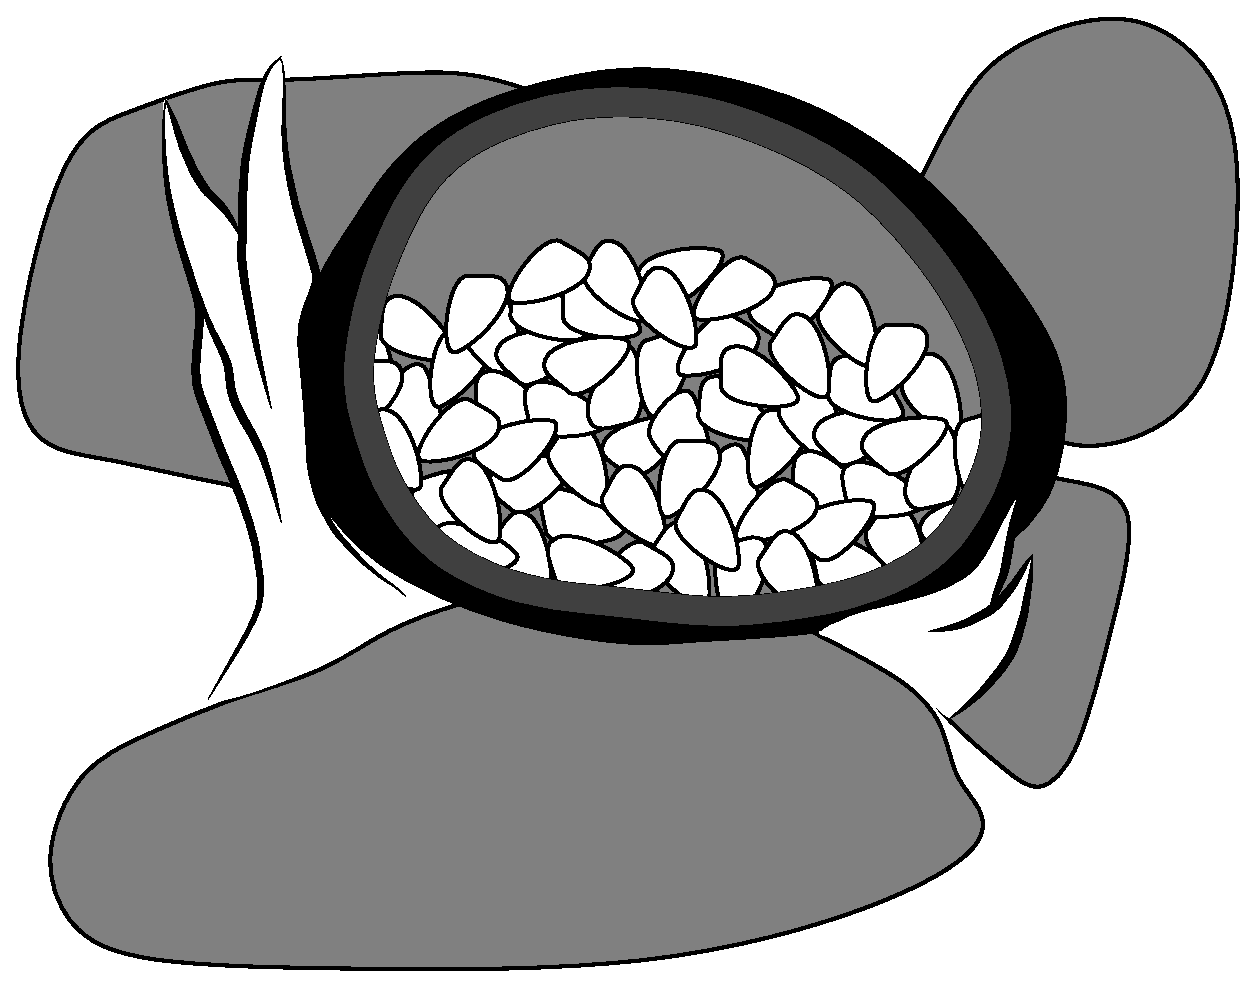
\includegraphics[width=0.47\textwidth]{cancha.eps}
  \end{center}
  \vspace{-20pt}
  %\caption{Zandor}
\end{wrapfigure}
Minha família não era endinheirada, e talvez esse conceito escapava a meu entendimento naquela época, mas nada do que realmente me importava me faltava.
Lembro que minha casa era de adobe e madeira com teto de telha. Minha mãe cozinhava sobre uma fogueira pequena, e minhas irmãs e eu, certamente, usávamos com muita frequência roupas que a simples vista qualquer pessoa consideraria que eram várias medidas menores das que precisávamos;
porém, para mim, minha casa era um castelo amplo e fresco, no qual eu ia descansar após voltar da escola ou do trabalho na chacra. 
A cozinha da minha mãe era a melhor; ela estava cheia de sabores obtidos dos mesmos produtos que cultivávamos ou cuidávamos. 
Em dias especiais, meu pai ia ao rio e comíamos peixe. Outras vezes, na estação seca, comíamos charque\footnote{Carne desidratada ao sol.} com alguma mistura de ovos de perdiz ou de galinha; dependendo da sorte do dia.
O queijo e o leite não faltavam nas nossas refeições; que tanto podiam ser de cabra ou de vaca.
As sobremesas dependiam da estação do ano, pois as frutas como figos-da-índia, pêssego, figo, melão-andino, sanky\footnote{Fruta dos Andes peruanos com múltiplos benefícios para a saúde.}, entre outras tinham cada uma sua temporada. Também tinham épocas para sobremesas elaboradas com milho fresco e outras com chila-caiota; com este último, minha mãe fazia meu mingau favorito. Era inacreditável para mim que: um creme de semelhante majestade podia ser construído com só um pouco de açúcar, canela, cravo e chila-caiota.

Minhas irmãs e eu gostávamos de brincar juntos, sair a passear procurando frutas e ir apreciar animais silvestres. Em geral, nós não tínhamos discussões importantes, porém devo reconhecer que: eu de quando em quando costumava fazer alguma maldade.
Nesses casos, elas recorriam às maiores autoridades da casa, com os senhores que governavam e decidiam sobre o bem e o mal, ou seja: meus pais. 
Lembro que, ao princípio, meu pai me falava com frases como: 
--- Aurelio, você não deve esconder a boneca da sua irmã. --- 
Se o assunto era mais grave ele dizia: 
--- Aule! Por que você colocou um grilo na cabeça da sua irmã? --- 
Se minha insistência na procura de problemas chegava a níveis perigosos para minha existência, meu pai gritava: 
--- Aulicha! Por que você colocou pimenta na balinha da sua irmã? ---
Assim, quando eu escutava meu pai me chamar de Aulicha, eu já sabia que minha sorte tinha sido decidida e que uma chicotada estava próxima. A ideia de fugir sempre passava por minha cabeça, porém minhas experiências anteriores me indicavam que isso só iria me prejudicar mais, e ia resignado diante do meu pai. Inclusive, em várias ocasiões, ele me pedia para levar o chicote de três pontas, pequeno e veloz, que era ao mesmo tempo um velho conhecido e meu principal antagonista.

A minha vida no campo sempre estava cheia de contrapontos, tantos eram os momentos tristes quanto os alegres, e algumas vezes, mais das que me permitiriam pensar que era só uma casualidade, os momentos tristes preparavam um caminho inevitável e irreversível às épocas alegres e vice-versa; como um ciclo que se retroalimenta para se manter perpétuo. 
Assim, uma das minhas maiores alegrias era souber que meu pai retornava de viagem, geralmente da costa do Peru, não só devido à saudade que deixava a partida dele e a alegria que trazia seu retorno, mas também porque ele voltava cheio de presentes. Ele nos trazia doces, bolachas, brinquedos, roupas e itens diversos; os quais, comumente, nós nos Andes não tínhamos acesso.
Por outro lado, entre meus momentos mais tristes, estava a perda de algum ente querido e a consequente impotência ao não ser capaz de evitar sua partida. 
No entanto, tudo isso é parte da vida e gostaria compartilhar com vocês alguns desses momentos.



%Ayacucho é uma cidade do distrito de Ayacucho, na província de Huamanga, no departamento de Ayacucho, no Peru
